% ================================================================== PART II
\part{Numerics: turning the equations into code}

\chapter{Finite differences and noise amplification}

\section{Stencils used everywhere}
All spatial derivatives use second-order finite differences on the uniform PIV grid (spacing $h$), including at the edges.

\begin{table}[H]\centering\small
\begin{tabular}{@{}llll@{}}\toprule
Quantity & Where & Stencil & Truncation error\\\midrule
$f'$ & interior & $(f_{i+1}-f_{i-1})/2h$ & $-\tfrac{h^2}{6}f'''$\\
$f'$ & left edge & $(-3f_0+4f_1-f_2)/2h$ & $+\tfrac{h^2}{3}f'''$\\
$f''$ & interior & $(f_{i+1}-2f_i+f_{i-1})/h^2$ & $-\tfrac{h^2}{12}f''''$\\
$f''$ & left edge & $(2f_0-5f_1+4f_2-f_3)/h^2$ & $+\tfrac{11h^2}{12}f''''$\\
$\partial_t f$ & middle snapshot & $(f^{n+1}-f^{n-1})/2\Delta t$ & $-\tfrac{\Delta t^2}{6}f_{ttt}$\\\bottomrule
\end{tabular}
\caption{The finite-difference stencils (\code{core/derivatives.py}). The right edge mirrors the left.}
\end{table}

\textbf{Deriving the one-sided first derivative.} Expand about $x_0$:
$f_1=f_0+hf'+\tfrac{h^2}{2}f''+\tfrac{h^3}{6}f'''$ and $f_2=f_0+2hf'+2h^2f''+\tfrac{4h^3}{3}f'''$.
Look for $(af_0+bf_1+cf_2)/h$ whose $f_0$ and $f''$ coefficients vanish and whose $f'$ coefficient is 1:
\[
a+b+c=0,\qquad b+2c=1,\qquad \tfrac b2+2c=0 \;\Rightarrow\; a=-\tfrac32,\; b=2,\; c=-\tfrac12 .
\]
The same procedure with four points (cancel $f_0,f',f'''$, keep $f''$) gives $(2,-5,4,-1)/h^2$.

\begin{pitfall}[Boundary stencils must be second order too]
The Neumann data $\n\cdot\G$ and the source term on the boundary rows are computed with these edge stencils. A first-order stencil there would pull the \emph{global} order of the whole reconstruction down to 1. (Chapter~11 shows this deliberately with \code{order=1}.)
\end{pitfall}

\section{How differentiation amplifies noise}
Suppose every velocity sample carries independent noise of standard deviation $s=\sigma U$. Linear combinations of independent errors add in variance:
\begin{align}
\text{time difference: }&\operatorname{std}\!\left[\frac{\epsilon^{n+1}-\epsilon^{n-1}}{2\Delta t}\right]=\frac{\sqrt2\,s}{2\Delta t}=\frac{s}{\sqrt2\,\Delta t},\\
\text{first derivative: }&\frac{s}{\sqrt2\,h},\\
\text{5-point Laplacian: }&\frac{\sqrt{1^2+1^2+1^2+1^2+4^2}\;s}{h^2}=\frac{\sqrt{20}\,s}{h^2}.
\end{align}
Putting these into $\G$:
\begin{equation}
\operatorname{noise}(\G)\sim \underbrace{\rho\frac{s}{\sqrt2\Delta t}}_{\partial\uu/\partial t}+\underbrace{\rho U\frac{s}{\sqrt2 h}}_{\text{convective}}+\underbrace{\mu\frac{\sqrt{20}\,s}{h^2}}_{\text{viscous}} .
\label{eq:noiseG}
\end{equation}

\begin{keyidea}[The central tension of the whole project]
Truncation error falls as $h^2$ and $\Delta t^2$, but noise amplification grows as $1/h$, $1/h^2$ and $1/\Delta t$. Refining the measurement therefore helps only up to a point. Below an optimum spacing the error \emph{rises} again. Minimising $E(h)\approx Ch^2+K\sigma/h^q$ gives $h_{opt}\propto\sigma^{1/(2+q)}$: noisier data need a coarser grid.
\end{keyidea}

\begin{figure}[H]\centering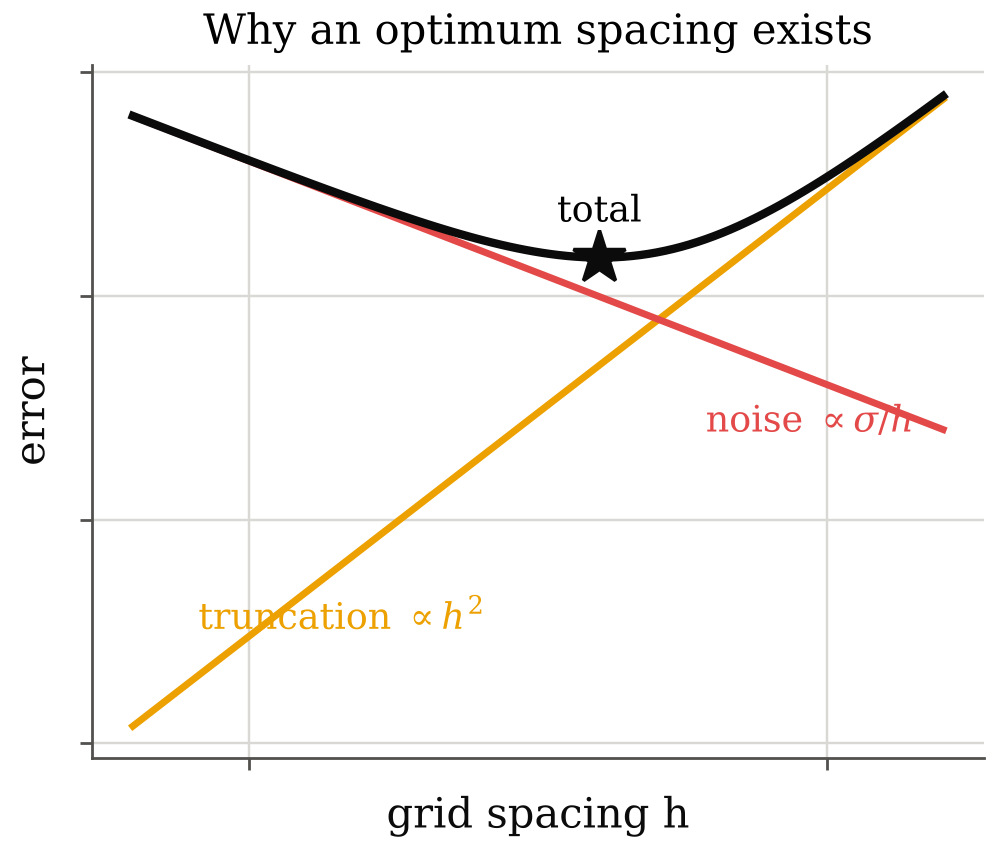
\includegraphics[width=0.45\linewidth]{img/f_tradeoff.png}
\caption{Error budget (schematic): truncation error falls with $h$, noise amplification rises, and the total has a minimum.}\end{figure}

% ------------------------------------------------------------------
\chapter{The discrete pressure-Poisson problem}

\section{The 5-point Laplacian}
Unknowns $p_{i,j}$ sit at the PIV nodes, numbered $k=j\,n_x+i$. In the interior,
\begin{equation}
\frac{p_{i+1,j}-2p_{i,j}+p_{i-1,j}}{\Delta x^2}+\frac{p_{i,j+1}-2p_{i,j}+p_{i,j-1}}{\Delta y^2}=f_{i,j}=(\nabla\cdot\G)_{i,j},
\end{equation}
with truncation error $-\tfrac{\Delta x^2}{12}p_{xxxx}-\tfrac{\Delta y^2}{12}p_{yyyy}$. The matrix is assembled with Kronecker products, $A=I_y\otimes D_{xx}+D_{yy}\otimes I_x$, and stored as a sparse CSR matrix.

\section{Neumann boundaries by ghost-point elimination}
At the left edge ($i=0$) invent a ghost node $i=-1$ outside the domain. Discretise the Neumann condition $\partial p/\partial x=G_x$ centrally:
\begin{equation}
\frac{p_1-p_{-1}}{2\Delta x}=G_{x,0}\quad\Rightarrow\quad p_{-1}=p_1-2\Delta x\,G_{x,0}.
\end{equation}
Substitute into the Laplacian row at $i=0$ and move the known part to the right-hand side:
\begin{equation}
\frac{2p_1-2p_0}{\Delta x^2}+[\,y\text{-part}\,]=f_0+\frac{2G_{x,0}}{\Delta x}.
\end{equation}
The other edges follow the same pattern: right edge $b\mathrel{-}=2G_x/\Delta x$, bottom $b\mathrel{+}=2G_y/\Delta y$, top $b\mathrel{-}=2G_y/\Delta y$. In 1-D the operator becomes the matrix with rows $[-2,\,2]$, $[1,-2,1],\dots,[2,-2]$, all divided by $h^2$.

\textbf{Corners} have two ghost neighbours, one in $x$ and one in $y$. Each is eliminated with \emph{its own} condition ($\partial p/\partial x=G_x$ and $\partial p/\partial y=G_y$), so both are used exactly. Averaging the two conditions (as the original project specification suggested) would throw information away.

\textbf{Order of accuracy.} The boundary rows have local truncation error $O(h)$, since $(2p_1-2p_0)/h^2-2g/h=p''+\tfrac h3p'''+\dots$ But the global error is still $O(h^2)$:
\begin{itemize}
\item the $O(h)$ error lives on a strip of width $O(h)$ only;
\item multiplying edge rows by $\tfrac12$ and corner rows by $\tfrac14$ turns the scheme into a vertex-centred finite-volume scheme on half and quarter cells, whose flux errors are $O(h^2)$.
\end{itemize}
The tests confirm global slopes of 1.8--2.2.

\textbf{Symmetric form.} With trapezoidal weights $w$ (1 inside, $\tfrac12$ on edges, $\tfrac14$ at corners) and $W=\operatorname{diag}(w)$, the matrix $WA$ is symmetric and $S=-WA$ is symmetric positive semi-definite. Conjugate gradients needs exactly this.

\section{The all-Neumann system is singular}
$A\mathbf{1}=0$: adding a constant to $p$ changes nothing, so $A$ has a one-dimensional null space and the pressure is fixed only up to a constant. The left null vector is $w$ ($w^TA=0$), so $Ap=b$ is solvable only if $w^Tb=0$, and
\begin{equation}
\Delta x\,\Delta y\,w^Tb=\text{trapezoidal}\iint f\,dA-\text{trapezoidal}\oint\n\cdot\G\,ds ,
\end{equation}
the \emph{discrete compatibility residual}. Two fixes are implemented:

\begin{description}[style=nextline]
\item[\code{pin="node"}: replace one row by $p_k=0$]
The system becomes solvable, but the discarded row was the only place the incompatibility $R$ could go. $R$ then acts as a point source at the pinned node, producing a logarithmic disturbance $\sim(R/2\pi)\ln r$ around it. Errors are larger: on clean Taylor--Green $5.8\times10^{-3}$ vs $7.2\times10^{-4}$.
\item[\code{pin="mean"} (default): zero-mean augmented system]
\begin{equation}
\begin{bmatrix}A&\mathbf 1\\\mathbf 1^T&0\end{bmatrix}\begin{bmatrix}p\\\lambda\end{bmatrix}=\begin{bmatrix}b\\0\end{bmatrix}
\quad\Longleftrightarrow\quad Ap+\lambda\mathbf 1=b,\;\;\textstyle\sum p=0.
\end{equation}
Multiplying the first row by $w^T$ gives $\lambda=w^Tb/w^T\mathbf 1$: a \emph{uniform} source correction spreads the incompatibility evenly instead of dumping it at one node. The bordered matrix is non-singular because $\mathbf1$ is not in the range of $A$ ($w^T\mathbf 1\neq0$).
\end{description}

\textbf{Dirichlet edges} (known pressure, from taps or Bernoulli) replace those rows by $p_k=$ value. Such an edge fixes the constant, so no pin is needed.

\begin{viva}
\begin{enumerate}[leftmargin=*]
\item \emph{Why is the all-Neumann matrix singular?} $A\mathbf 1=0$; fix it by pinning a node or adding a zero-mean constraint.
\item \emph{Why is pin-mean better than pin-node?} Pin-node dumps the incompatibility $R$ at one point (a point source); pin-mean spreads it uniformly.
\item \emph{What does $\lambda$ represent?} The uniform source correction that makes the data compatible.
\item \emph{Why is the global error second order if boundary rows are first order?} The $O(h)$ error acts only on an $O(h)$ strip; equivalently the scaled scheme is a second-order finite-volume scheme.
\end{enumerate}
\end{viva}

% ------------------------------------------------------------------
\chapter{Direct and omni-directional integration}

\begin{figure}[H]\centering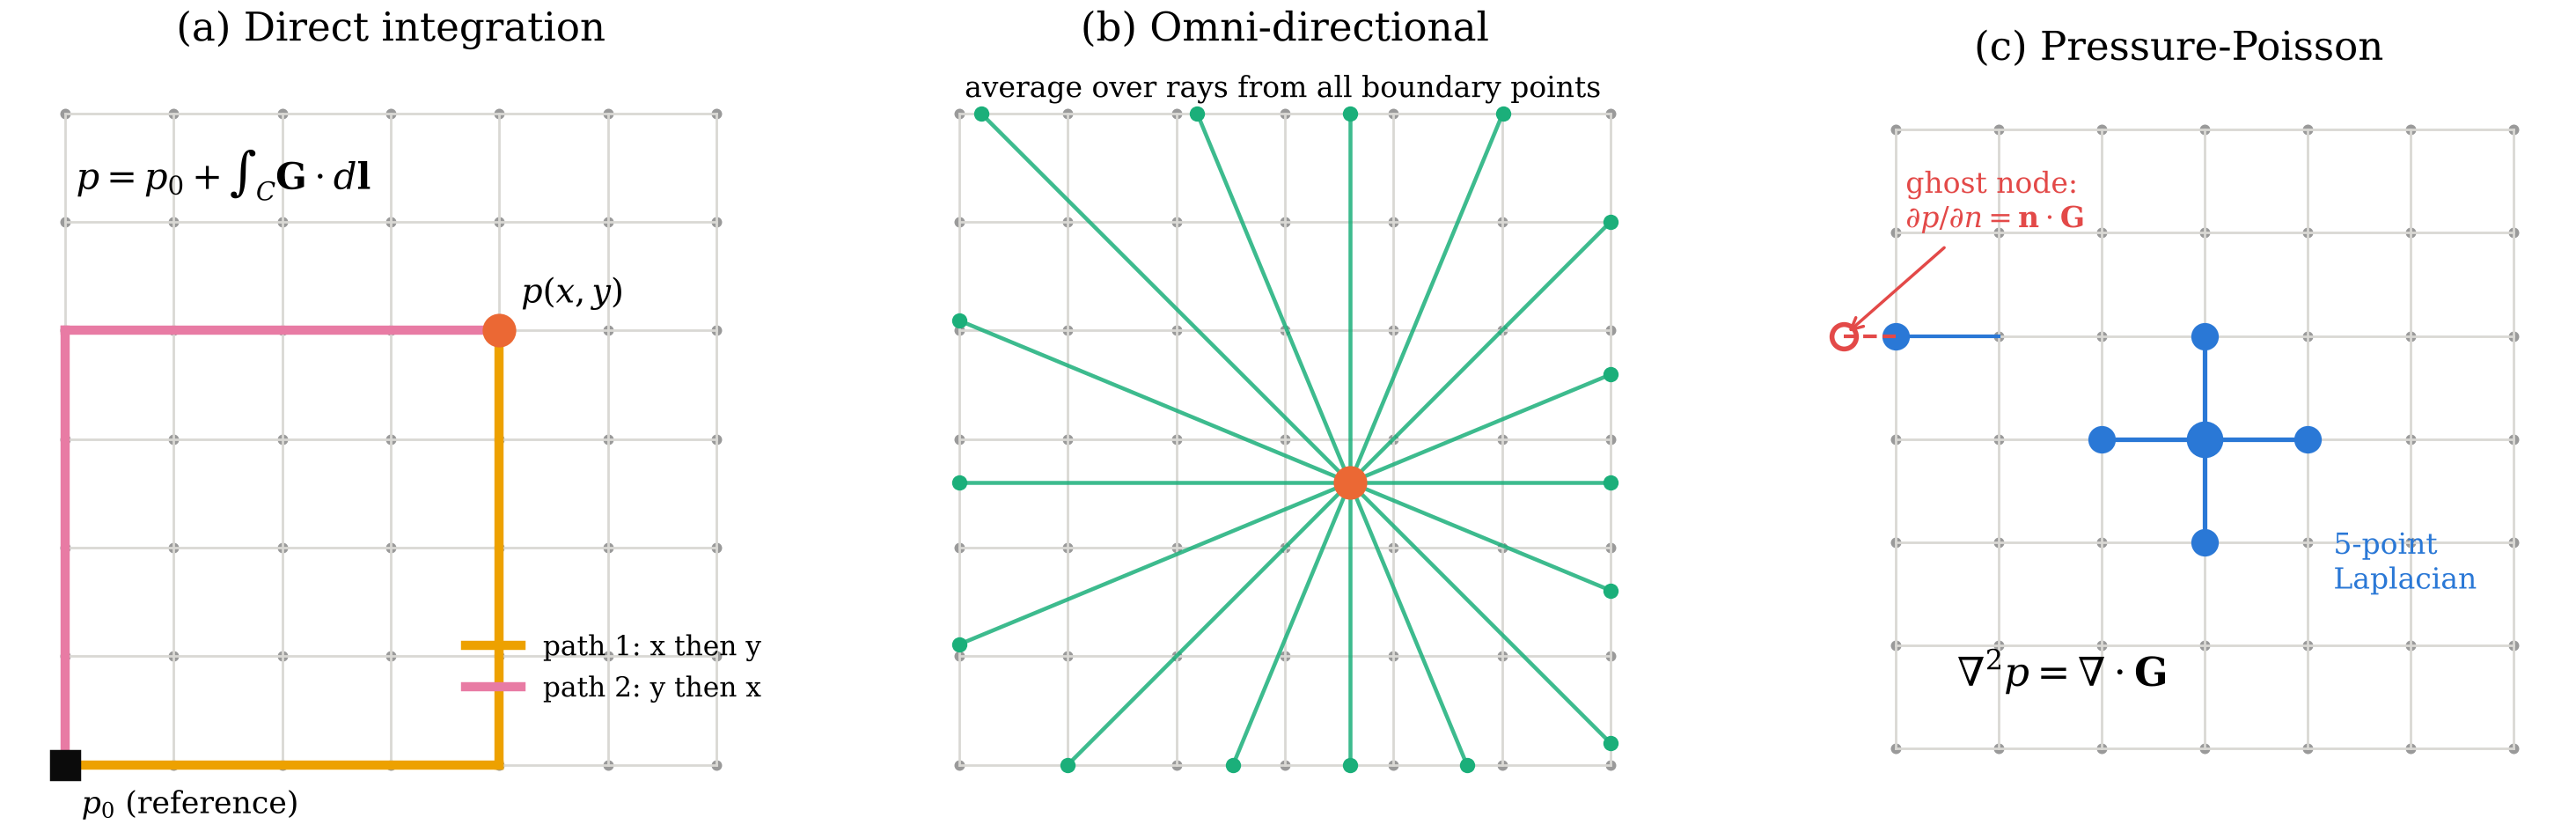
\includegraphics[width=\linewidth]{img/f_methods.png}
\caption{The three algorithms on the PIV grid: (a) direct integration along two paths, (b) omni-directional rays from all directions, (c) the Poisson stencil with a ghost node.}\end{figure}

\section{Direct spatial integration}
The simplest idea: integrate the gradient along a path from a reference point,
\begin{equation}
p(B)-p(A)=\int_A^B\G\cdot d\mathbf l,
\end{equation}
using the cumulative trapezoidal rule (second order).
\begin{itemize}
\item \textbf{Path 1:} along the first row in $x$, then up each column in $y$.
\item \textbf{Path 2:} along the first column in $y$, then along each row in $x$.
\item The code reports both and their average.
\end{itemize}
For an exact gradient both paths agree (Stokes: $\oint\G\cdot d\mathbf l=\iint\operatorname{curl}\G\,dA=0$). Measured $\G$ has a curl, so they differ; the difference measures path dependence.

\begin{keyidea}[Why direct integration is so noise-sensitive]
Along a path of $N=L/h$ steps the trapezoidal sum adds $N$ independent errors of size $h\,\sigma_G$. They add like a random walk: error $\propto h\,\sigma_G\sqrt{N}=\sigma_G\sqrt{hL}$. With $\sigma_G\sim s/h$ from the derivatives this is $\propto s\sqrt{L/h}$, which \emph{grows} as the grid is refined, and faster still where the viscous noise $\sim s/h^2$ matters. Every error made early on the path is carried to every later point.
\end{keyidea}

\section{Omni-directional integration}
Liu \& Katz (2006) proposed averaging line integrals over many paths from all directions, so that path errors cancel. The project implements a \emph{rotating-ray} variant (\code{core/omni\_integration.py}):
\begin{enumerate}
\item Directions $\theta_k=2\pi k/N$, $k=0,\dots,N-1$, with $N=32$.
\item From every node $P$, trace a straight ray backwards to the boundary point $E_k(P)$ and integrate $\G\cdot\mathbf e_k$ from $E_k$ to $P$ (trapezoidal rule, step $h$, bilinear interpolation of $\G$).
\item \textbf{Boundary stage.} Boundary values depend on each other through the rays: $p_i=\operatorname{mean}_k\big[\sum_mA_{im}p_m+I_i\big]$, i.e.\ a linear system $(I-A)p_b=c$. Its null space is the constants and it is not exactly compatible (curl $\G\neq0$), so it is solved with the same zero-mean augmented system as above.
\item \textbf{Interior stage.} $p(P)=\operatorname{mean}_k\big[p_b(E_k)+\int\G\cdot\mathbf e_k\,ds\big]$.
\end{enumerate}
The original paper uses a virtual boundary with parallel rays and iterates the boundary values. This version keeps the principle (many directions, boundary values consistent with the rays) but starts the rays at each node.

\textbf{Cost.} $O(N\times\text{nodes}\times\text{ray length})$: about 0.4\,s at $64^2$ against 15\,ms for Poisson. That is why the noisy grid study runs omni only up to $64^2$.

% ------------------------------------------------------------------
\chapter{Iterative solvers, norms and convergence}
The default Poisson solver is a sparse direct factorisation (\code{scipy.sparse.linalg.spsolve}). The course (Lecture 11) asks how iterative solvers behave, how to judge convergence, and how to measure residuals. The project implements all of this on the same matrix.

\section{Norms of a residual}
For a residual vector $r$ with $n$ entries:
\begin{table}[H]\centering\small
\begin{tabular}{@{}lll@{}}\toprule
Norm & Formula & Meaning\\\midrule
$L_1$ & $\sum|r_i|$ & total absolute imbalance\\
$L_2$ & $\sqrt{\sum r_i^2}$ & Euclidean length; large entries dominate\\
$L_\infty$ & $\max|r_i|$ & worst cell only\\
$L_{1n}$ & $\tfrac1n\sum|r_i|$ & mean imbalance per cell\\
$L_{2n}$ & $\sqrt{\tfrac1n\sum r_i^2}$ & RMS imbalance per cell\\
scaled & $L_{2n}(r)/S$ & relative imbalance ($S=L_{2n}(b)$)\\\bottomrule
\end{tabular}\end{table}
For a residual of constant size $c$ on $n$ cells, $L_1=nc$ and $L_2=\sqrt n\,c$ grow with the grid while $L_{1n}=L_{2n}=c$ do not. A fixed tolerance on an unnormalised norm is therefore harder to meet the finer the grid; the project measures exponents 0.99 ($L_1$) and 0.50 ($L_2$) vs about 0 for the normalised norms. Always $L_{1n}\le L_{2n}\le L_\infty$.

\emph{Lecture example} (a unit test): $r=(0.0001,0.0004,0.0006,0.002)$ gives $L_1=0.0031$, $L_2=0.00213$, $L_{2n}=0.00106$.

With $p^0=0$ the first residual is $b$, so the scaled residual starts at exactly 1, and ``tol $=10^{-8}$'' means ``reduce the imbalance by $10^8$''.

\section{Jacobi is pseudo-time marching}
Jacobi updates $p^{k+1}=p^k+\omega D^{-1}(b-Ap^k)$ with $D=\operatorname{diag}A$. For $\Delta x=\Delta y=h$ every diagonal entry is $-4/h^2$, so
\begin{equation}
p^{k+1}=p^k+\underbrace{\omega\frac{h^2}{4}}_{\Delta\tau}\left(\nabla_h^2p^k-f\right),
\end{equation}
which is explicit Euler time-stepping of the pseudo-transient equation $\partial p/\partial\tau=\nabla^2p-f$ toward its steady state $\nabla^2p=f$.

\textbf{Stability.} Each eigenmode is multiplied by $1+\Delta\tau\lambda$, with $\lambda\in[-8/h^2,0]$ for the 5-point Laplacian. Stability needs $|1-8\Delta\tau/h^2|\le1$, i.e.\ $\Delta\tau\le h^2/4$, which is exactly classic Jacobi ($\omega=1$).

\begin{pitfall}[Classic Jacobi stalls on the all-Neumann problem]
At $\Delta\tau=h^2/4$ the checkerboard mode $(-1)^{i+j}$ (eigenvalue $-8/h^2$) is multiplied by $-1$ every step: it flips sign and never decays. With all-Neumann walls the checkerboard is an \emph{exact} eigenvector, so the residual levels off at a floor ($4.2\times10^{-8}$ at $64^2$, above tol $10^{-8}$). The project uses $\omega=0.95$ by default (amplification $-0.9$), which converges at a 5\,\% cost.
\end{pitfall}

\textbf{Convergence rate.} The smoothest mode decays by $1-\omega\mu_{min}$ per step with $\mu_{min}\approx(\pi h/L)^2/4$. Reducing the residual by a factor $F$ takes about $\ln F/\mu_{min}\propto(L/h)^2\propto N$ iterations: Jacobi's count grows linearly with the number of unknowns.

\section{Gauss--Seidel and SOR}
Gauss--Seidel uses the newest values as soon as they are available; SOR over-relaxes the update by $\omega$. The code uses \textbf{red-black ordering} (all nodes with $i+j$ even, then all odd), which vectorises each half-sweep and is ``consistently ordered'', so Young's theory applies:
\begin{itemize}
\item $\rho_{GS}=\rho_J^2$: Gauss--Seidel needs half the Jacobi iterations (measured 12\,328 vs 25\,366 at $64^2$).
\item SOR is optimal at $\omega_{opt}=2/\big(1+\sqrt{1-\rho_J^2}\big)$ with $\rho_{SOR}=\omega_{opt}-1$; the iteration count then scales like $\sqrt N$ instead of $N$.
\end{itemize}
\textbf{Neumann vs Dirichlet.} The textbook formula $\omega_{opt}=2/(1+\sin(\pi h/L))$ assumes Dirichlet walls ($\rho_J=\cos\pi h/L$). With all-Neumann walls the slowest non-constant mode varies in one direction only, $\rho_J=\cos^2(\pi h/2L)$, so the optimum is larger: 1.932 instead of 1.905 at $64^2$. The measured best $\omega$ is 1.9319 (314 iterations); the Dirichlet formula needs 628.

\textbf{Kahan's theorem:} $\rho_{SOR}\ge|\omega-1|$, so SOR cannot converge for $\omega\ge2$. The project shows $\omega=2$ (no decay) and $\omega=2.1$ (divergence to $10^{10}$ in 145 iterations).

\section{Conjugate gradient}
CG minimises the error in the energy norm over a growing Krylov space. It needs a symmetric positive (semi-)definite matrix, so it runs on $S=-WA$ (same equations, rows scaled by their trapezoidal weights) with a Jacobi preconditioner. Its iteration count scales like $\sqrt{\kappa(S)}\sim L/h\propto\sqrt N$. For the singular zero-mean problem it converges from $p^0=0$ because the right-hand side is made compatible.

\section{Residual vs change: when is a solution converged?}
For Jacobi, $p^{k+1}-p^k=\omega D^{-1}r^k$, so $\|p^{k+1}-p^k\|=\Delta\tau\|r^k\|$ with $\Delta\tau\approx3\times10^{-4}$ at $64^2$: the change is $10^3$--$10^4$ times smaller than the residual. Worse, the true error is $\|p^k-p^*\|\approx\|p^{k+1}-p^k\|/(1-\rho)$, and $1/(1-\rho)$ is huge when convergence is slow.

\begin{keyidea}[Do not stop on a small change alone]
A small change per iteration does \emph{not} mean convergence when convergence is slow. In the project, the change first drops below $10^{-6}$ at iteration 6\,697 while the scaled residual is still $6.1\times10^{-4}$ and the true error $1.7\times10^{-3}$. The solvers therefore stop on the scaled residual. The same logic applies to declaring a CFD run ``steady''.
\end{keyidea}

\begin{viva}
\begin{enumerate}[leftmargin=*]
\item \emph{Show that Jacobi is explicit pseudo-time marching.} $D^{-1}=-h^2/4$, so $p^{k+1}=p^k+\Delta\tau(\nabla^2_hp^k-f)$ with $\Delta\tau=\omega h^2/4$.
\item \emph{Why does classic Jacobi stall here but not with Dirichlet walls?} The Neumann checkerboard mode has amplification exactly $-1$; Dirichlet walls shift the extreme eigenvalue inside the stable range.
\item \emph{Why is SOR so much faster?} Over-relaxation moves the spectral radius from $1-O(h^2)$ to $1-O(h)$: iterations $\propto\sqrt N$ instead of $N$.
\item \emph{Why not use CG on $A$ directly?} $A$ (ghost-point form) is not symmetric; $-WA$ is.
\item \emph{Why normalise residual norms?} So that the same physical imbalance gives the same number on any grid.
\end{enumerate}
\end{viva}
